\documentclass{article}
\usepackage[backend=biber]{biblatex}
\usepackage{graphicx}
\usepackage[colorlinks=true]{hyperref}
\usepackage{booktabs}
\usepackage{siunitx}
\usepackage[]{amsmath}
\usepackage{gensymb}
\usepackage{mathtools}
\usepackage{fancyref}
\usepackage{chemfig}
\addbibresource{/home/giorgio/Bibliography/bibliography.bib}
\hypersetup{
    colorlinks=true,
    linkcolor=blue,
    filecolor=magenta,  
    citecolor=blue,    
    urlcolor=cyan,
    pdftitle={Selective Laser Sintering for sustainable polymers},
    bookmarks=true,
}

\author{Giorgio De Trane}
\title{\textbf{Selective Laser Sintering for sustainable polymers}}

\begin{document}
    \setlength{\parindent}{0pt}
    \maketitle
    \begin{center}
        
\includegraphics[width=0.8\textwidth]{Pictures/polito_logo.eps}\linebreak\newline
        \textit{Year 2021/2022}
    \end{center}

    \newpage
    \tableofcontents
    \newpage
    \section{Introduction\label{Intro}}

    \textit{Additive manufacturing} (AM) is a broad term that encompasses several manufacturing techniques, characterized by their additive nature, as the name suggests, 
    in contrast with more traditional subtractive processes.
    
    AM techniques are applied to a vast range of materials, including ceramics, polymers and metal alloys, some of which are specifically developed or optimized to 
    these kinds of applications. \\ 
    
    The main advantage of AM is the ability to produce complex shapes in a relatively short time. 
    These geometries are either too hard or even impossible to reproduce with subtractive manufacturing techniques, which often require multiple steps, using different 
    pieces of equipment, trained personnel, etc. \\

    Given the same material, the complex shapes allowed by AM can replace components made of multiple assembled parts with a unique solid piece of comparable or even better mechanical properties. 
    
    The inherent flexibility of AM often allows product designers to simplify or even entirely bypass the very strict CAD workflow (which is intrinsically tied to 
    traditional manufacturing processes) and make use of organic and/or generative modeling. 

    As a consequence of better design choices and minimal need of post-processing of AM objects, far less raw material is wasted, compared to subtractive manufacturing techniques, leading to 
    long term lowering of costs, faster design-to-market pipelines and, last but not least, lower emissions and environmental impact \autocite*{Recent_progress_polymers_AM}. 

    \subsection{Polymers in Additive Manufacturing\label{Polymers_in_AM}}

    Polymers and their composite materials have been used in all sorts of fields, ranging from arts and crafts all the way to advanced biomedical and aerospace applications, thanks 
    to their unique and varied extended range of properties. \\  
    
    The rapid advancement of AM, where polymers have been extensively used for prototyping, in the form of resins, filaments, powders and viscous inks, 
    has increased the demand for high-performance polymers, in order to take advantage of their quicker printing times (compared to metals) as well as their lower cost, while still
    maintaining good mechanical properties for an end product, rather than just a prototype \autocite*{Recent_progress_polymers_AM}. \\ 

    The urge for drastically reducing the environmental impact of human activities involves every production field, including AM, which can be inherently less impactful
    than traditional manufacturing processes, given the same material and final product to achieve. 

    A consequence of the concerns about climate change and its potentially catastrophic outcomes is the research in the field of eco-friendly materials, including polymers 
    that could be used in AM. 
    
    A great example is \textit{PLA} (PolyLactic Acid), a polymer widely used in 3D printing, whose monomer is obtained by fermenting starches, such as corn starch. \\ 

    Many new eco-friendly polymers have been and are currently being studied for AM techniques, but this case study will focus mostly on materials that can be potentially turned 
    into powders for \textit{PBF} (Powder Bed Fusion) techniques or filaments for \textit{ME} (Material Extrusion). 
    
    \subsection{Common AM techniques for polymers\label{AM_techniques_summary}}
    
    Polymers can be processed with several AM techniques, including, but not limited to: 

    \begin{itemize}
        \item \textbf{VP} (Vat Photopolymerization), which make use of UV lights (or other radiations) to solidify photosensitive resins. This class of AM processes can produce 
                        parts with the highest resolution among all AM methods \autocites*{Recent_progress_polymers_AM}{Kovalcik_PHA_Review};
        \item \textbf{MJ} (Material Jetting), which consist of a deposition of viscous fluids (either in droplets or in a continuous fashion), solidified by different agents 
                            (time interacting chemicals, heating, cooling, drying, photopolymerization, etc.). These processes include several patented methods, characterized by 
                            high speed printing \autocite*{Recent_progress_polymers_AM};
        \item \textbf{PBF} (Powder Bed Fusion), where the object is printed by locally fusing a powder bed (with a pulsing energy source -such as lasers- or with a local deposition of chemicals),
                            layed out in a layer-by-layer fashion \autocites*{Recent_progress_polymers_AM}{Kovalcik_PHA_Review};
        \item \textbf{ME} (Material Extrusion), where each layer is printed by direct deposition of materials through a nozzle, that solidify as they cool down \autocites*{Recent_progress_polymers_AM}{Kovalcik_PHA_Review};
        \item \textbf{BJ} (Binder Jetting), similarly to 2D inkjet printing utilizes a
                        polymer in the form of a liquid binder, that gets deposited in droplets onto a powder bed (usually made of metallic or ceramic particles). This 
                        method can build large parts without support structures and the lack of a high power heat source cuts its cost down, but the structural 
                        properties of the final parts are poor compared to sinterized equivalents, making heat treatments necessary \autocite*{Recent_progress_polymers_AM};
        \item \textbf{Sheet Lamination}, where thin sheets of material are stacked together and bonded with adhesives or heat. This class of techniques 
                        is not entirely additive, since subtractive processes are used to cut and refine the final part, creating substantial material waste \autocite*{Recent_progress_polymers_AM}.
    \end{itemize} \clearpage

    \subsubsection{FDM (Fused Deposition Modeling) \label{FDM_general}}

    FDM is a ME technique and the most well known AM process, commonly named 3D printing in popular media. \\
    
    The process consists of a direct layer-by-layer deposition of a thermoplastic filament, heated up to its melting point (or enough to soften it until it reaches an 
    optimal flow) and extruded through a nozzle \autocites*{Recent_progress_polymers_AM}{Kovalcik_PHA_Review}. 

    The nozzle is generally moved in the x-y plane until a layer is completed with the desired infill, then either the extruder head or the growth plate are moved along the z axis, 
    initiating the printing of the subsequent layer.

    The planar infill and the resolution on the z axis will determine the quality of the final print for a given material and geometry, in terms of density and visual appeal.
    
    For a given planar infill, the z axis resolution greatly influences the final look of the part, as well as printing times:
    modern slicing software can analyze the geometry and generate an adaptive resolution, reducing the number of layers where the local  
    curvature of the object is within a certain threshold and increasing it when necessary. 
    
    This approach can produce good quality parts, 
    while reducing printing times. \\ 
    
    FDM has gained a lot of popularity in the last few years, given its general ease of use, relatively low cost of both materials and equipment and its growing 
    community of enthusiasts. \\

    A wide variety of materials can be used with this technique, including (but not limited to) 
    \textit{PLA}, \textit{ABS}, \textit{PET}, \textit{PETG}, \textit{HIPS}, \textit{TPU}, \textit{nylon}. \clearpage

    \subsubsection{SLS (Selective Laser Sintering) \label{SLS_general}}

    \textit{SLS} is a manufacturing process in the PBF family. 

    A powder bed is layed out onto a platform and a focused heat source (a laser) locally sinterizes the powder, 
    until a single layer is completed \autocites*{Recent_progress_polymers_AM}{Kovalcik_PHA_Review}. 

    A mechanism swipes out the remaining powder, which is recollected and automatically redistributed by a recoating 
    system for each subsequent layer \autocite*{Padovano_SLS_Review}. 

    This process is similar to \textit{SLM} (Selective Laser Melting), typically used with metal alloys: in \textit{SLS} the energy input is not high enough 
    to bring the powders to their melting point, but sufficient for sinterization of the powders. 

    Despite the slight difference, many sources use the terms interchangeably, often effectively referring to SLM. 
    
    When it comes to thermoplastic materials, the required laser power to melt each layer is substantially lower than that needed for metals. \\ 

    \textit{SLS} printers can be considerably more expensive than \textit{FDM} machines of similar printing volume, but the advantages they offer, 
    in terms of customizability, superior consistency in print quality and accuracy, higher production rate, less need for support structures, 
    makes them a more cost effective solution for larger scale industrial production, whereas \textit{FDM} printers are still more established 
    in the hobbyists and enthusiasts market \autocite*{Padovano_SLS_Review}. \\ 

    Generally speaking, \textit{SLS} is a three stage process, consisting of: 
    
    \begin{itemize}
        \item warm up (A)
        \item building (B)
        \item cooling (C)
    \end{itemize}

    \begin{figure}[h!]
        \centering
        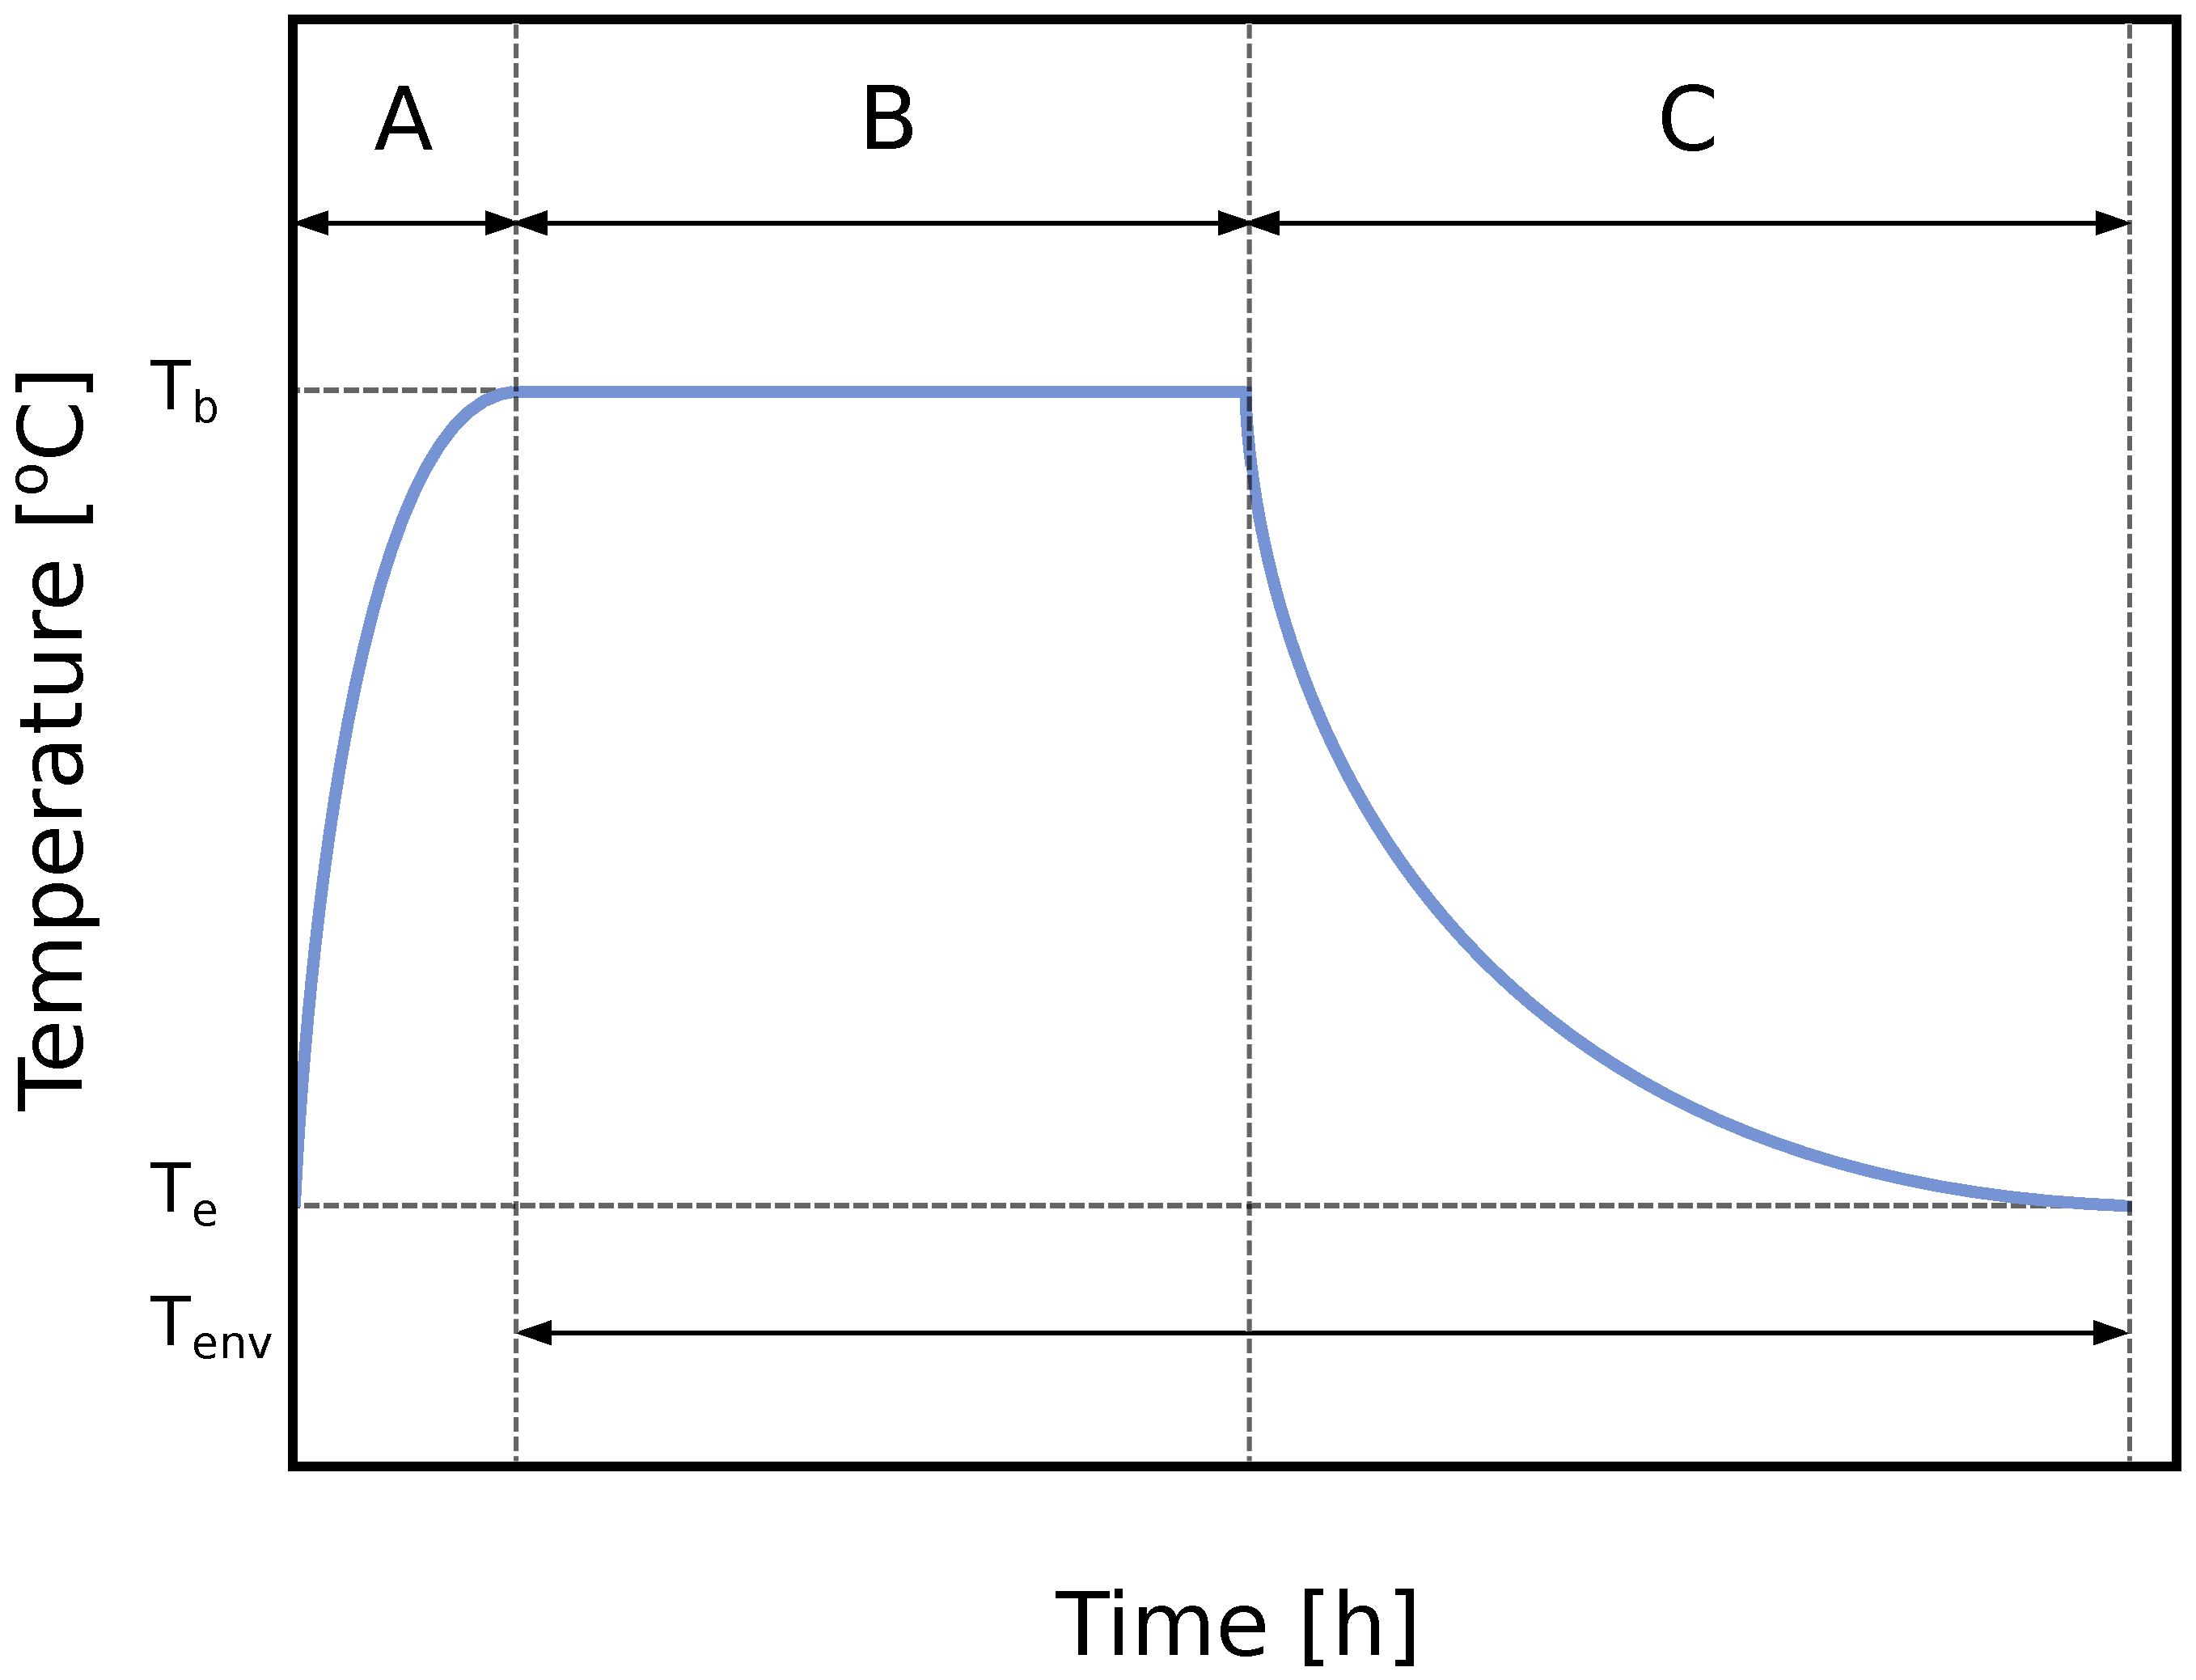
\includegraphics[width=0.63\textwidth]{Pictures/SLS_temp_over_time.eps}\\
        \caption{Phases of an \textit{SLS} process \autocites{Inkscape}{Padovano_SLS_Review}} 
        \label{fig:SLS_temp_over_time}
    \end{figure}

    As seen in figure (\ref{fig:SLS_temp_over_time}), the first phase is the time required to reach a specific powder bed temperature $(T_b)$, based on the chosen material. 

    Ideally this temperature should be maintained constant inside the printing
    chamber, during the entire printing phase, through infrared or electric heaters. 
    
    The main goal is avoiding drastic temperature gradients in different areas of the printed part, since they can cause 
    visual artefacts such as local or global deformation and, most importantly, uneven residual mechanical tension that can 
    rapidly degrade the structural integrity of the final piece, especially in structural components that might be placed under static or
    dynamic loads. \\ 
    
    Once the final piece is printed, the entire chamber is cooled down homogeneously and gradually, until the equilibrium is reached at room 
    temperature $(T_e)$ \autocite*{Padovano_SLS_Review}. \\ 

    Quality standards for \textit{SLS} printed parts have increased dramatically over the last few years, to the point where 
    the manufactured components are not exclusively used for prototyping or as sacrificial items for investment casting, but they are 
    used as finalized industrial grade parts. 

    However, there is still room for substantial improvements in the consistency of print accuracy, overall quality, reliability 
    and scalability of the entire process, compared to more traditional manufacturing techniques. \\ 

    The variety of physical phenomena involved in SLS, the fact that they can be interdepent and their different temporal regimes are the main 
    source of complexity that makes the process very hard to study and inconsistent. 

    The most predominant phenomena are the following \autocite*{Padovano_SLS_Review}: 

    \begin{itemize}
        \item Laser motion and irradiation
        \item Thermal diffusion
        \item Polymer viscous flow and particle coalescence 
        \item Powder spreading
        \item Solidification/crystallization 
    \end{itemize} 
    
    Further improvements are required in order to reduce the amount of discarded parts (still comparatively 
    higher than most consolidated manufacturing techniques), usually defective in terms of porosity or 
    thermal distortion or warping \autocite*{Padovano_SLS_Review}. \\ 

    The next chapters will focus on potential SLS materials for this case study and their powder production specifically. \clearpage

    \section{PHAs (Polyhydroxyalkanoates)  \label{PHA_in_general}}

    \textit{PHA}s are a family of thermoplastic polyesters, obtained by hydroxyalkanoic acids via bacterial fermentation, under 
    nutrient depletion and carbon excess conditions \autocites{Kovalcik_PHA_Review}{Messori_Bondioli_PHAs}. 

    They are a sustainable alternative to petrochemical polymers commonly utilized in 
    additive manufacturing and they are mostly used for prototyping in the medical field \autocites{Kovalcik_PHA_Review}{Messori_Bondioli_PHAs}. 

    Similarly to other sustainable plastics, \textit{PHA} can be produced using industrial byproducts as substrates (corn, soy, coffee, oil wastes, etc.)
    \autocite{Kovalcik_PHA_Review}. \\ 

    The monomer composition of PHA can be very diverse, depending on the microorganisms involved and the fermentation medium. 
    
    This variety impacts the overall mechanical, thermal and chemical properties of the final plastic, which depend on the concentration of 
    different monomers in polymers and copolymers. 

    PHAs can be classified by the chain-length of their monomers \autocite*{Messori_Bondioli_PHAs}: 

    \begin{itemize}
        \item \textit{scl-PHA} (short-chain-length PHA) with 3 to 5 carbon atoms
        \item \textit{mcl-PHA} (medium-chain-length PHA) with 6 to 14 carbon atoms
        \item \textit{lcl-PHA} (long-chain-length PHA) with more than 14 carbon atoms
    \end{itemize}


    Estimating the exact meaningful measures of these properties is not always a straight-forward process, 
    since manufacturers are not transparent about the exact composition of their products, which may be 
    improved by additives, whose percentage is not often fully disclosed \autocite{Kovalcik_PHA_Review}. \\ 
    
    The market for bioderived PHA has gradually increased over the years and the growth is estimated to keep its pace, given that not only are they more sustainable
    to competing petrochemical polymers, but they offer additional valuable properties, such as piezolectricity 
    and protection against gases and UV lights \autocite{Kovalcik_PHA_Review}.

    Their bio-origin, non-toxicity, renewability, biodegradability and biocompatibility make PHAs a very compelling product in the 
    ever growing market of sustainable materials. 

    However, these desirable qualities are a contributing factor to their higher price, which is still not competetive with more established 
    polymers of similar properties \autocite{Kovalcik_PHA_Review}. 

    The increasing demand and the improvements on their biosynthesis will make their price more accessible in the future, for all sorts of 
    applications, including additive manufacturing, where PHAs can be printed successfully either with FDM or SLS techniques. \clearpage

    
    \subsection{PHA and Additive Manufacturing \label{PHA_in_Additive}}

    PHAs can be used in different AM techniques, including Stereolitography, which is part of VP processes (\ref{AM_techniques_summary}), 
    Fused Deposition Modeling (\ref{FDM_general}), where the filaments are made of a mixture of PHA and PLA, 
    (which increases thermal stability and cuts down cost), and 
    Selective Laser Sintering (\ref{SLS_general}) \autocite{Kovalcik_PHA_Review}. \\ 

    This case study will focus on its usage in SLS. \\ 

    PHAs have been successfully printed via SLS and utilized in the medical field as scaffolds for tissues engineering applications. 

    These scaffolds can be printed with a porous structure (controlled by the laser energy density), 
    which could carry biomolecules and release drugs, for instance.
    
    Unlike with FDM applications, where PHA can not be used as a standalone filament, but needs PLA addition in order to stabilize its melting 
    phase, PHA powders in SLS maintain a good stability and their chemical composition does not get altered as easily. 

    This is a clear advantage, since the overall properties of the final products do not change drastically from its starting powder, 
    and, in addition to this, the remaining powder is not thermally altered close to the melting pool, meaning that it can 
    be reused for additional printing \autocite{Kovalcik_PHA_Review}.  \\
        
    \subsubsection{PHBH \label{PHBH}}

    Can't find anything RN \clearpage

    \section{PBS (Polybutylene Succinate) \label{PBS_in_general}}

    \section{PBAT (Polybutylene Adipate Terephtalate) \label{PBAT_in_general}}

    \section{Powder production for SLS \label{Powder_production}}

    Manufacturing raw materials for FDM is a relatively easy process, since the plastics need to be mass produced into filaments or pellets \ref{FDM_general}.

    Producing powders from plastics is a much harder process. \\ 

    Two radically different approaches are possible, each with its own critical issues: 

    \begin{itemize}
        \item Chemical precipitation
        \item Mechanical milling
    \end{itemize}









    \clearpage

    \printbibliography
    
\end{document}